%
% teil1.tex -- Beispiel-File für das Paper
%
% (c) 2020 Prof Dr Andreas Müller, Hochschule Rapperswil
%
% !TEX root = ../../buch.tex
% !TEX encoding = UTF-8
%
\section{Modellbildung
\label{openfoam:section:teil1}}
\kopfrechts{Modellbildung}
Zum Simulieren von Strömungen benötigen wir zum einen ein Modell das das verhalten des Mediums, im Fall einer Strömungssimulation eine Flüssigkeit, dass das Verhalten des Mediums möglichst umfassend und genau beschreibt. 
Hierbei werden meist die Navier Stokes Gleichungen benutzt welche noch mit der Kontinuitätsgleichung und Energiegleichung erweitert jedoch werden auch in einigen Fällen die Euler Gleichungen oder die Potentialgleichungen verwendet da diese zwar ein weniger vollständiges Modell beschreiben jedoch weniger Rechenintensiv sind.

Zudem benötigen wir ein Lösungsverfahren das Einen Anfangszustand und das Mathematische Modell zu einer Numerischen Lösung verarbeiten kann dies ist nötig da für die Navier Stokes Gleichungen keine Analytische Lösung existiert und die der Euler Gleichungen sehr aufwendig sind zu berechnen. 
Hierbei kommen meist die Finite-Differenzen-Methode (FDM), die Finite-Volumen-Methode (FVM)und die Finite-Elemente-Methode (FEM) zum Einsatz. 

OpenFoam nutzt dabei meist die Finite-Volume-Methode dies ist jedoch eines der Gebiete in dem sich OpenFOAM von anderen Simulations Programmen unterscheidet da es sich Besonders dafür eignet Neue algorithmische Lösungsverfahren zu implementieren und zu testen.

\subsection{Stationär oder Zeitabhängig?}
Bei der Strömungsmechanik wird zuerst unterschieden ob es sich um eine Stationäre oder Zeitabhängige Strömung handelt.
Das heisst es ist entweder der Fall dass an jedem Ort im Raum die Geschwindigkeit der sich dort befindenden Flüssigkeit in Bezug auf Betrag und Richtung konstant ist (Stationär) oder dass sich diese Grösse ändert (Zeitabhängig).
Bei einer Simulation wird meist Simuliert bis der Stationäre zustand, bis auf einen kleinen Fehler, erreicht wird.
Dadurch kann man sich Simulationsaufwand ersparen da sobald der Stationäre zustand erreicht wird das Resultat nicht mehr ändert und so keine neuen Ergebnisse gefunden werden können.

\subsection{Modellierung der Flüssigkeit}
Im Kontext der CFD Simulation nimmt man an dass eine Flüssigkeit nicht aus einzelnen Teilen wie Atome oder Moleküle besteht, sondern man nimmt an dass die Flüssigkeit kontinuierlich, also ohne Zwischenräume, ist. 
Zudem wird angenommen dass sämtliche Eigenschaften die sich von Punkt zu Punkt innerhalb der Flüssigkeit Kontinuierlich und die Ableitung davon ebenfalls Kontinuierlich sind. 

Zudem hat eine Flüssigkeit noch weitere Eigenschaften wie die Dichte diese kann hier aber nicht immer als Konstant angesehen werden da man ansonsten bei kompressiblen Flüssigkeiten einen grossen teil der Energie nicht beachten würde.
Zudem muss die Viskosität und die spezifische Wärmekapazität, wobei die Viskosität in der Navier-Stokes Gleichung benötigt wird.

\subsection{Die Euler Gleichungen}
Die Euler Gleichungen beschreiben das verhalten der Strömung eines reibungsfreien Fluides, also eines Laminaren Flusses dessen Reibung vernachlässigt werden kann. 
Das bedeutet sie können nicht für alle Probleme eingesetzt werden da sobald Reibungskräfte einen substantiellen Einfluss auf die Strömung haben, das Berechnete Ergebnis eine zu grosse Abweichung aufweist.

\subsubsection{Massenerhaltung}
Die Erste Euler Gleichung geht aus der Idee hervor dass man ein beliebiges Volumen $V$ hat, das fest im Raum liegt. Durch ein Oberflächenstück 
$d \vectorbold{S} $ 
des Volumens 
$V$
 fliesst jeweils der Massenstrom 
$\vb{S} \cdot\rho\vb{u}$.
Aus dem Massenstrom des Oberflächensegments kann man dann mit dem Oberflächenintegral 
\[\int_{S}d\vb{S}\cdot\rho\vb{u}\]
den Gesamten Massenstrom berechnen. Dieser Massenstrom muss nun gleich sein wie die Massenänderung der in dem Volumen enthaltenen Flüssigkeit 
\[\frac{\partial M}{\partial t}\]
dies lässt sich mit dem Integral 
\[\int_{V}\frac{\partial \rho}{\partial t} dV\]
berechnen, hier integriert man die Dichteänderung in einem Volumenelement über das ganze Volumen 
$V$ 

Setzt man nun die beiden Terme gleich erhält man die Gleichung 
\[\int_{S}d\vb{S}\cdot\rho\vb{u} 
=
\int_{V}\frac{\partial \rho}{\partial t} \, dV ,\] 
bei dieser Gleichung kann man nun auf der L.H.S. mit dem Gaussschen Integralsatz das Oberflächen Integral in ein Flächenintegral umwandeln es wird also zu
\[\int_{V}\nabla\cdot(\rho\vb{u}) 
=
\int_{V}\frac{\partial \rho}{\partial t} \, dV \]
mit dem ändern der Flussrichtung und umschreiben der Gleichung kann man die R.H.S auf Null setzen und die Integrale zu einem Integral
\[\int_{V}\frac{\partial \rho}{\partial t} + \nabla\cdot(\rho\vb{u})  \, dV 
= 
0\]
zusammenfassen.

Dies kann nun in einem letzten Schritt in die Differentialgleichung
\[\frac{\partial \rho}{\partial t} + \nabla\cdot(\rho\vb{u})  \, dV 
= 
0\] 
umwandeln.

\subsubsection{Impulserhaltung}
Bei der Impuls Erhaltung geht man fast gleich vor wie beim herleiten der Gleichung für die Massenerhaltung.
Man geht ebenfalls von einem beliebigen Volumen Flüssigkeit, $V$, das nicht mehr fest an Ort und beliebigem Masseninhalt ist ,sondern eine feste menge Masse die sich durch den Raum bewegt.
Dieses Volumen weist nun eine Impulsänderung die 
\[\frac{D}{Dt}\int_{V}\rho\vb{u}\, dV\]
entspricht.

Als nächstes berechnet man die gesamte kraft auf die Oberfläche des Volumens $V$ in dem man alle Kräfte $\vb{f} = \vb{t}\,dS$, die auf die Oberflächenstücke $dS$ wirken, integriert.
Wobei $\vb{t} dS$ gleich $(\vb{n\cdot\sigma}dS)$ ist. 
Daraus erhält man die Kraft 
\[\vb{Fs} 
=
\int_{S}\vb{f}\, dS
= \int_{S} (d\vb{S}\cdot\vb{\sigma})
\]
Dies ist nun wieder ein Flächenintegral das mit dem Gaussschen Integralsatz in ein Volumenintegral umgewandelt werden kann.
Dadurch ergibt sich dass
\[\vb{Fs} 
=
\int_{V}\nabla \cdot \vb{\sigma}\, dV
.\]

Zuletzt berechnen wir noch den Einfluss anderer Kräfte wie die Schwerkraft auf den Impuls des Volumens $V$.
Dazu integrieren wir den Vektor $\vb{b}$, bei dem es sich um eine Beschleunigung handelt, über alle Volumenstücke $dV$ wodurch wir das Integral
\[\vb{Fa} 
=
\int_{V}\rho\vb{b}, dV
\]
erhalten.

Nun können wir die Impulsänderung des Volumens gleich der Summe der darauf wirkenden Kräfte setzen und die Integrale in einem Integral zusammenfassen, daraus erhalten wir, mit der Bedingung die Masse im Volumen sei konstant, die Gleichung 
\[\int_{V} \rho \frac{D\vb{u}}{Dt} - \nabla \cdot \vb{\sigma} -\rho \vb{b}\, dV
=
0
\]
hierbei kann man das Integral wider weglassen wodurch wir die Differentialgleichung
\[\rho \frac{D\vb{u}}{Dt}
= 
\nabla \cdot \vb{\sigma} +\rho \vb{b}
\]
erhalten.

Zuletzt kann man noch die substantielle Ableitung in eine partielle umwandeln damit wir die gleiche Form wie für die Massenerhaltungs Gleichung erhalten.
Dazu nutzen wir die Definition der substantiellen Ableitung
\[
\frac{D\Phi(\vb{x},t)}{Dt}
:=
\frac{\partial \Phi}{\partial t}+(\vb{u}\cdot \nabla)\Phi
\] 
eingesetzt in die Differentialgleichung erhalten wir so 
\[ \rho\frac{\partial\vb{u}}{\partial t} + \nabla \cdot(\rho\vb{u}\vb{u})
= 
\nabla \cdot \vb{\sigma} +\rho \vb{b}.
\]
Diese Form erleichtert einem die Berechnung da sie nicht mehr die Impulsänderung einer sich bewegenden Menge Flüssigkeit beschreibt sondern die Impulsänderung der sich momentan an einem Ort befindenden Masse. Man kann also anstelle ein sich durch den Raum bewegendes Masseteilchen ein Festes Volumenelement Simulieren welches bei der Fluiddynamik-Simulation die bevorzugte Methode ist.

\subsubsection{Energieerhaltung}
Die Dritte der Euler Gleichungen wurde nicht wie die der Masse und Impulserhaltung von Leonhard Euler hergeleitet, sie wird jedoch auch als  Euler Gleichung bezeichnet.

Das Gesetz der Energieerhaltung besagt dass die Gesamte Energie in einem isolierten System Konstant bleibt .
Die Dritte Euler Gleichung beschreibt dieses Naturgesetz mit der Differentialgleichung 
\[\rho \frac{De}{Dt}+  \rho \frac{DK}{Dt}
=
- \nabla \cdot \vb{q} + \rho r + \nabla \cdot (\sigma \cdot \vb{u} + \rho \vb{b} \cdot \vb{u} )
\]
, welche besagt dass die Änderung der thermischen Energie $\rho \frac{De}{Dt}$ und die der kinetischen $\rho \frac{DK}{Dt}$ (wobei $K$ die kinetische Energie $\frac{\abs{\vb{u}}^{2}}{2}$ ist) zusammen die gesamte Änderung der Energie im Volumenelement $V$ sind.
Diese Gesamte Energieänderung wird aus dem Zufluss Mechanischer und Thermischer Energie, aber auch durch Hitze und Mechanische Leistungsquellen im inneren des Volumens, berechnet.
So ist der Zufluss, ins innere des Volumen, aus den Termen $- \nabla \cdot \vb{q}$ und $\nabla \cdot (\sigma \cdot \vb{u})$ welche den Zufluss Thermischer respektive Mechanischer Energie durch die Oberfläche des Volumens darstellen.
Dazu kommt noch die Änderung der Energie durch Quellen im Inneren des Volumens durch Hitzequellen $\rho \vb{q}$ und Mechanische Energiequellen $\rho \vb{b} \cdot \vb{u}$.




\subsection{Navier-Stokes}
%TODO !!!!!!!!!!!!!!!!!!!!!!!!!!!!!!!!!!!!!!!!!!!!!!!!!!!!!!!!!!!!!!!!!!!!!!!!!!!!!!!!!!!!!!!!!!!!!!!!!!!!!!!!!!!!!!!!!!!!!!!!!!!!¨
\subsection{Objekt Modellierung}
Bei der CFD Simulation müssen nicht nur die Physikalischen Eigenschaften des Mediums, sondern auch die Form des Objektes dessen Influenz auf die Flüssigkeit und die Umgebung in der sich das Objekt befindet simuliert werden soll Modelliert werden.
Dazu gehören zum einen die Geometrischen Eigenschaften des Objektes und die Umgebung in dem es sich befindet, zudem aber auch die Eigenschaften wie die Oberflächen der Objekte mit der Flüssigkeit interagieren.

Zum modellieren der Objekte kann man eine beliebige CAD Software benutzen, für OpenFOAM muss dieses Modell dann jedoch konvertiert werden.
Dazu ist eine Software, snappy hex  mesh, die bei OpenFOAM beinhaltet ist verfügbar.
Sie verarbeitet das 3D Modell, meist im STL Format, zusammen mit einem simpleren Modell für die Begrenzung der Lösungs-Domain, welches für OpenFoam bei simplen Geometrien am beste im blockMesh Format definiert wird, zusammen um zum einen die Form der Lösungs-Domain (Raum in der sich die Flüssigkeit in der Simulation befindet) zu generieren und zudem eine Diskretisierung der Flächen und Unterteilung des Raumes in Zellen.
Diese Diskretisierung ist benötigt dass die Finite Volume Methode verwendet werden kann um das Mathematische Modell der Flüssigkeit auf der Lösungs Domain anzuwenden.
Ein Beispiel dafür ist in Bild \ref{openfoam:fig:SD_Modell_vergleich} zu sehen.
\begin{figure}[h]
	\centering
	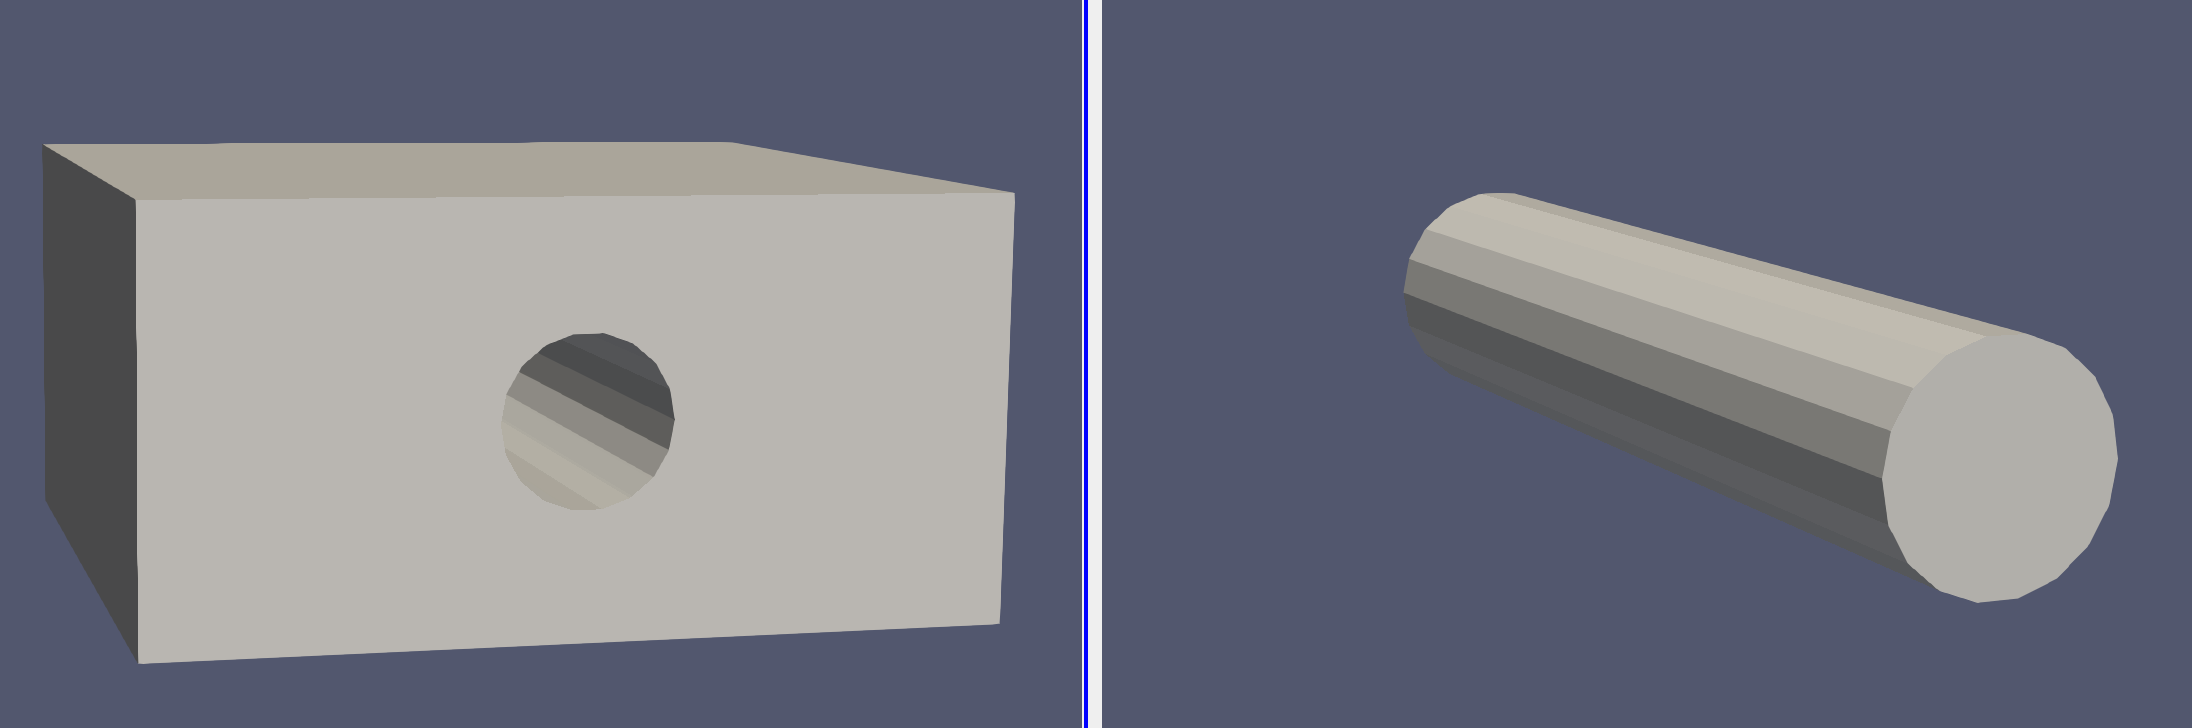
\includegraphics[scale=0.1]{papers/openfoam/Bilder/vergleich_solution_domain_object.png}
	\caption{Vergleich der Solution Domain (L) und dem 3D Modell des Objektes (R)}
	\label{openfoam:fig:SD_Modell_vergleich}
\end{figure}

In Bild \ref{openfoam:fig:sim_grid} ist zudem ein Beispiel für die Unterteilung der Geometrie in Zellen zu sehen.
Darauf sieht man einen weiteren Vorteil des Gitters, es wird nahe dem Objekt nämlich die Grösse der Zellen verringert.
Dadurch kann der Rechenaufwand der ansonsten betrieben werden muss um die ganze Lösungsdomain mit dem feineren Gitter zu lösen, das wir für genügend Detail am Objekt benötigen, verringert werden.

\begin{figure}[h]
	\centering
	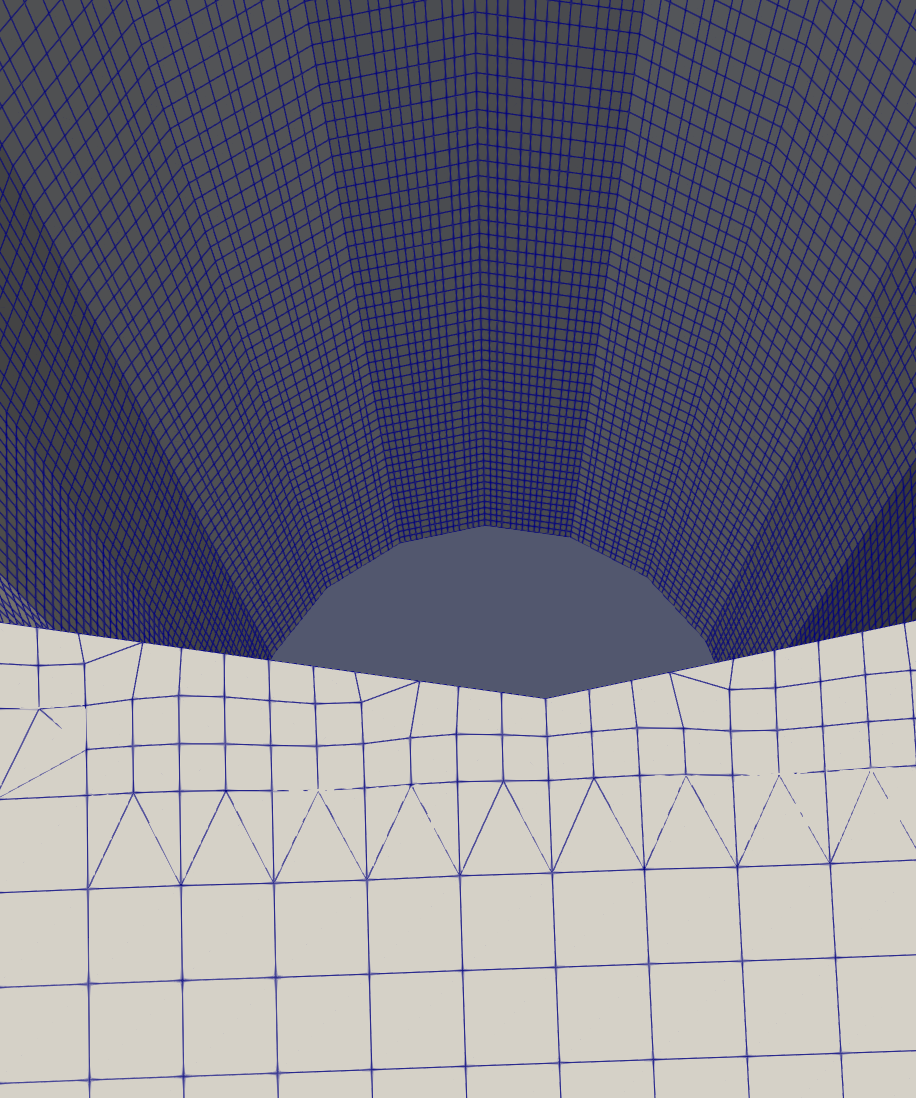
\includegraphics[scale=0.1]{papers/openfoam/Bilder/grid.png }
	\caption{Beispiel des Rechengitters das von Snappy Hex Mesh generiert wird}
	\label{openfoam:fig:sim_grid}
\end{figure}
 Zudem ist auch zu sehen dass die Zellen nicht unbedingt Würfel sein müssen das Netz kann theoretisch aus beliebigen Polyeder bestehen,  dies ist aber nicht unbedingt vorteilhaft denn es ist anzustreben ein Seitenverhältnis der Zellen von ungefähr 1 zu wählen dies spart Zeit beim verarbeiten der 3D Modellen zum Mesh.

%TODO Prozess in Ordnerstruktur beschreiben
